\documentclass[c,unicode,russian]{beamer}
\usepackage{hyperref}
\usepackage{alltt}
\usepackage{verbatim}
\usepackage{fancyvrb}

\usepackage{fontspec}
\setsansfont{Ubuntu}
\setmonofont{Ubuntu Mono}
\usepackage{polyglossia}
\setdefaultlanguage{russian}

\useinnertheme{metropolis}
\useoutertheme{metropolis}
\usecolortheme{metropolis}

\usepackage{listings}   % C++ code
\usepackage{xcolor}     % C++ code
\lstset{%
    keywordstyle=\color{blue},
    commentstyle=\color[rgb]{0.13,0.54,0.13},
    backgroundcolor=\color{yellow!10},
    basicstyle=\small\tt,
    stringstyle=\color{red}\ttfamily,
    belowcaptionskip=-1pt,
    xleftmargin=-15pt,
    framexleftmargin=-15pt,
    framexrightmargin=5pt,
    framextopmargin=5pt,
    framexbottommargin=5pt,
    framesep=0pt,
    rulesep=0pt
}
\lstdefinestyle{cpp}{%
    language=C++,
    morecomment=[l][\color{magenta}]{\#}
}
\lstdefinestyle{python}{%
    language=Python
}

\usepackage{caption}
\renewcommand{\lstlistingname}{Код} % Listing -> Algorithm
\DeclareCaptionFont{white}{\color{white}}
\DeclareCaptionFormat{listing}{\colorbox{gray}{\parbox{\textwidth}{#1#2#3}}}
\captionsetup[lstlisting]{format=listing,labelfont=white,textfont=white}

% logo of my university
\titlegraphic{\hspace{-1cm}
\includegraphics[width=2.5in]{../../_static/logo.jpg}}

\date{}
\author{Основы Веб-программирования}
\institute{Кафедра Интеллектуальных Информационных Технологий, ИнФО, УрФУ}

\usepackage{array}      % Table
\usepackage{dirtytalk}  % say
\usepackage{tabularx}

\title{Веб без фреймворков}

\begin{document}

% Slide #1
\frame{\titlepage}

% Slide #2
\begin{frame}{Ресурсы}
  \url{http://lectures.uralbash.ru/6.www.sync/2.codding/index.html}
\end{frame}

% Slide #3
\begin{frame}{WSGI - это\ldots?}

    Для разработки сайтов или Web-приложений на языке Python был утверждён
    стандарт взаимодействия между Python-приложениями и сервером (например
    Apache), названный WSGI (“Web Server Gateway Interface”).

    \textbf{Python}\newline
    \textbf{pep-333}\newline
    \textbf{pep-3333}\newline

\end{frame}

% Slide #4
\begin{frame}{Общие принципы}

  \begin{itemize}
    \item Веб-сервер
    \item Разделение кода: \textbf{MVC}, \textbf{MTV}, \textbf{RV}
    \item Маршрутизация URL
    \item Шаблоны
    \item Пагинация
    \item Request/Response
    \item Статика
    \item Формы
  \end{itemize}

\end{frame}


% Slide #7
\begin{frame}{Веб-сервер}

  \textbf{Веб сервер}

\end{frame}


% Slide #5
\begin{frame}{Веб-сервер}

  Задача Веб сервера - запускать Веб приложения.\newline\newline
    Популярные WSGI Веб сервера:\newline

  \begin{itemize}
    \item wsgiref
    \item Paste
    \item Waitress
    \item Gunicorn
  \end{itemize}


\end{frame}

% Slide #6
\begin{frame}[fragile]{wsgiref}

    \begin{lstlisting}[style=python]
    from wsgiref.simple_server import make_server

    def hello_world_app(environ, start_response):
        status = '200 OK'  # HTTP Status
        headers = [
          ('Content-type', 'text/plain; charset=utf-8')
        ]  # HTTP Headers
        start_response(status, headers)

        # The returned object is going to be printed
        return [b"Hello World"]

    with make_server('', 8000, hello_world_app) as httpd:
        print("Serving on port 8000...")

        # Serve until process is killed
        httpd.serve_forever()
    \end{lstlisting}

\end{frame}


% Slide #7
\begin{frame}{Разделение кода: \textbf{MVC}, \textbf{MTV}, \textbf{RV}}

  \textbf{Разделение кода на части}

\end{frame}


% Slide #7
\begin{frame}{Разделение кода: \textbf{MVC}}

  \textbf{MVC} (Model-View-Controller: модель-вид-контроллер) —

  шаблон архитектуры ПО, который подразумевает разделение программы на 3
  слабосвязанных компонента, каждый из которых отвечает за свою сферу
  деятельности.

\end{frame}


% Slide #8
\begin{frame}{Разделение кода: \textbf{MVC}}

  \begin{center}
    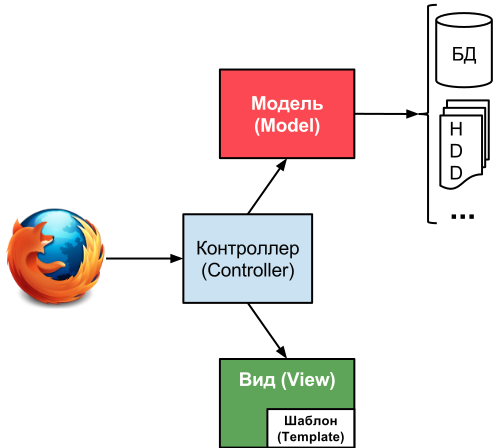
\includegraphics[width=3.2in]{media/mvc.png}
  \end{center}

\end{frame}


% Slide #9
\begin{frame}{Разделение кода: \textbf{MVC}}

  Классические \textbf{MVC} фреймворки:

  \begin{itemize}
    \item Ruby on Rails
    \item Pylons
  \end{itemize}

\end{frame}


% Slide #8
\begin{frame}{Разделение кода: \textbf{MTV}}

  Фреймворк \textbf{Django} ввел новую терминологию \textbf{MTV}

  \begin{itemize}
    \item \textbf{M -> M} Модели остались неизменными
    \item \textbf{V -> T} Представление назвали Templates
    \item \textbf{C -> V} Контроллеры назвали Views
  \end{itemize}

\end{frame}


% Slide #8
\begin{frame}{Разделение кода: \textbf{MTV}}

  Tada! Django MTV

  \begin{center}
    
\includegraphics[width=2.2in]{media/mtv_logo.jpg}
  \end{center}

\end{frame}

% Slide #8
\begin{frame}{Разделение кода: \textbf{MTV}}

  \begin{center}
    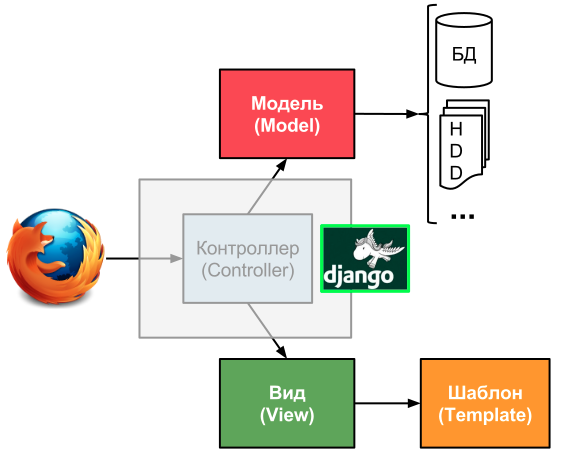
\includegraphics[width=3.2in]{media/mtv.png}
  \end{center}

\end{frame}

% Slide #11
\begin{frame}{Разделение кода: \textbf{MVC}, \textbf{MTV}, \textbf{RV}}

  Разработка без фреймворков дает вам возможность придерживаться любой
  архитектуры приложения и паттерна проектирования.

\end{frame}

% Slide #12
\begin{frame}{Разделение кода: \textbf{MVC}, \textbf{MTV}, \textbf{RV}}

  Это дает неоспоримую гибкость таким приложениям, оставляя ответственность по
  структуре ПО за разработчиком.

\end{frame}


% Slide #10
\begin{frame}{Разделение кода: \textbf{RV}}

  \textbf{RV} (Resources-View) --

  дает ту же гибкость, накладывая минимальную архитектуру идеально
  вписывающуюся в ограничения Веб приложений.

\end{frame}


% Slide #8
\begin{frame}{Разделение кода: \textbf{RV}}

  \begin{center}
    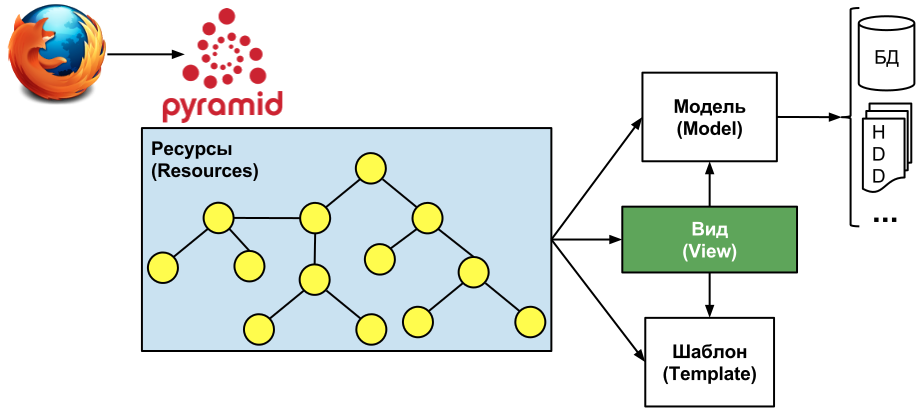
\includegraphics[width=4.0in]{media/rv.png}
  \end{center}

\end{frame}


% Slide #10
\begin{frame}{Разделение кода: \textbf{RV}}

  \say{Мы считаем, что есть только две вещи: ресурсы (\textbf{Resource}) и
    виды (\textbf{View}). Дерево ресурсов представляет структуру сайта, а вид
    представляет ресурс.
  }

\end{frame}

% Slide #10
\begin{frame}{Разделение кода: \textbf{RV}}

  \say{«\textbf{Шаблоны}» (\textbf{Template}) в реальности лишь
    деталь реализации некоторого вида: строго говоря, они не обязательны, и вид
    может вернуть ответ (Response) и без них.
  }

\end{frame}

% Slide #10
\begin{frame}{Разделение кода: \textbf{RV}}

  \say{Нет никакого «\textbf{Контроллера}» (\textbf{controller}): его просто не
    существует. «\textbf{Модель}» (\textbf{Model}) же либо представлена деревом
    ресурсов, либо «доменной моделью» (domain model) (например, моделью
    \textbf{SQLAlchemy}), которая вообще не является частью каркаса. Нам
    кажется, что наша терминология более разумна при существующих ограничениях
    веб-технологий.
  }

\end{frame}


% Slide #10
\begin{frame}{Разделение кода: \textbf{RV}}

  \textbf{Pyramid} only

    
\includegraphics[width=0.5in]{media/pyramid.png}

\end{frame}

% Slide #7
\begin{frame}{Маршруты}

  \textbf{Маршруты}

  или

  \textbf{Диспетчеризация URL}

\end{frame}

% Slide #8
\begin{frame}{Маршруты: Сортировочная Ж/Д станция}

  \begin{center}
    \vspace{-20pt}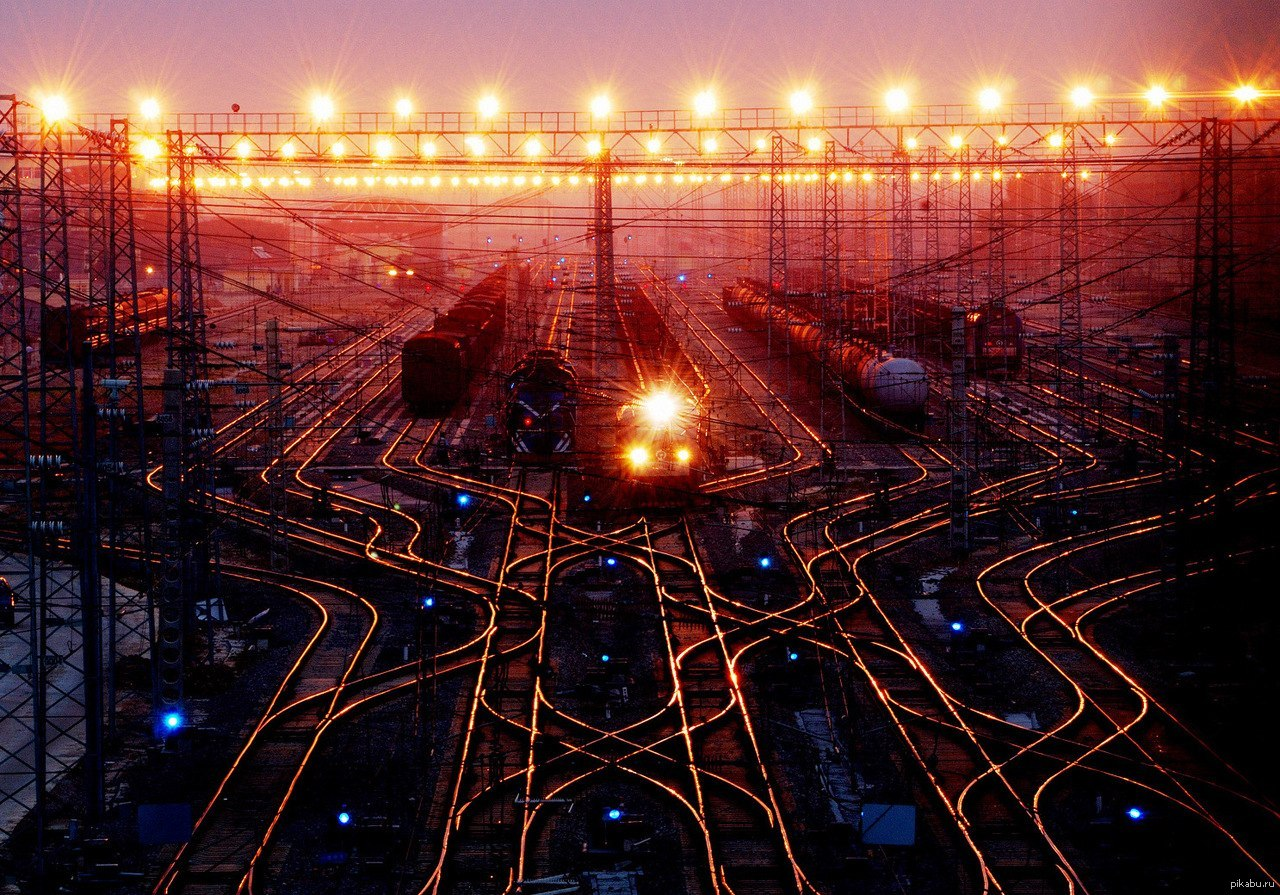
\includegraphics[width=\textwidth,height=\textheight,keepaspectratio]{media/routes.jpg}
  \end{center}

\end{frame}


% Slide #8
\begin{frame}{Маршруты: Сортировочная Ж/Д станция}

  \begin{itemize}
    \item \textbf{Поезда} похожи на HTTP запросы клиентов
    \item \textbf{Сортировочная станция} представляет из себя
      \textbf{маршруты}, только вместо поездов занимается диспетчеризацией HTTP
      запросов от клиентов
    \item \textbf{Пункт назначения} (завод или вокзал) можно сравнить с
      функцией (кодом), которая обрабатывает запрос
  \end{itemize}

\end{frame}


% Slide #8
\begin{frame}{Маршруты: Определение}

  \textbf{Маршруты} определяют шаблоны URL и связывают их со своим кодом

\end{frame}


% Slide #8
\begin{frame}{Маршруты: Преимущества}

  В отличии от CGI, где все привязано к файловой системе,
  если вы измените свое решение по поводу конкретного URL, то просто поменяйте
  шаблон URL - код по-прежнему будет работать отлично и не понадобится менять
  какую-либо логику.

\end{frame}

% Slide #8
\begin{frame}[fragile]{Маршруты: Регулярные выражения}

  \begin{lstlisting}[style=python]
    from django.conf.urls import url

    from . import views

    urlpatterns = [
     url(r'^articles/2003/$', views.special_case_2003),
     url(r'^articles/([0-9]{4})/$', views.year_archive),
     url(r'^articles/([0-9]{4})/([0-9]{2})/$', views.month_archive),
     url(r'^articles/([0-9]{4})/([0-9]{2})/([0-9]+)/$', views.article_detail),
    ]
    \end{lstlisting}

\end{frame}

% Slide #8
\begin{frame}[fragile]{Маршруты: Django 2.0 - Сопоставление с образом}

  \begin{lstlisting}[style=python]
    from django.urls import path

    from . import views

    urlpatterns = [
      path('articles/2003/', views.special_case_2003),
      path('articles/<int:year>/', views.year_archive),
      path('articles/<int:year>/<int:month>/', views.month_archive),
      path('articles/<int:year>/<int:month>/<slug:slug>/', views.article_detail),
    ]
    \end{lstlisting}

\end{frame}

% Slide #8
\begin{frame}[fragile]{Маршруты: Сопоставление с образом}

  \begin{lstlisting}[style=python]
    import selector

    dispatch = selector.Selector()
    dispatch.add('/', GET=BlogIndex)
    dispatch.add('/add', GET=create, POST=create)
    dispatch.add('/{id:digits}', GET=BlogRead)
    dispatch.add('/{id:digits}/edit', GET=update, POST=update)
    dispatch.add('/{id:digits}/delete', GET=delete)
  \end{lstlisting}

\end{frame}





\begin{frame}[fragile]{Маршруты: Сравнение}

  \begin{table}[]
  \centering
  \label{my-label}
  \begin{tabular}{ll}
    Регулярные выражения & Сопоставление с образом \\
    / & / \\
    /article/add & /article/add \\
    \verb|^/article/(?P<id>d+)/$|       & \verb|/article/{id:digits}|      \\
    \verb|^/article/(?P<id>d+)/edit$|   & \verb|/article/{id:digits}/edit| \\
    \verb|^/article/(?P<id>d+)/delete$| & \verb|/article/{id:digits}/delete|

  \end{tabular}
  \end{table}

\end{frame}

% Slide #8
\begin{frame}{Маршруты: Преимущества}

  \begin{itemize}
    \item
      Регулярные выражения дают огромные возможности.
    \item
      Но из-за ограничений \newline
      описанных в стандарте RFC 1738,
      большинство из них не нужны.
    \item
      Использование регулярных выражений затрудняет читабельность кода.
  \end{itemize}

\end{frame}


% Slide #8
\begin{frame}{Шаблоны}

  \textbf{Шаблоны}

\end{frame}


% Slide #8
\begin{frame}{Шаблоны: Определение}

  \textbf{Шаблоны} имеют очень простое определение - в статические файлы вставляются
  куски кода, при прогоне таких файлов через специальный транслятор
  (препроцессор), код заменяется результатом его выполнения.

\end{frame}


% Slide #8
\begin{frame}[fragile]{Шаблоны: C++}

  \begin{lstlisting}[style=cpp]
    template< typename T >
    T min( T a, T b )
    {
      return a < b ? a : b;
    }
  \end{lstlisting}

  \begin{lstlisting}[style=cpp]
    int min( int a, int b )
    {
      return a < b ? a : b;
    }

    long min( long a, long b )
    {
      return a < b ? a : b;
    }
  \end{lstlisting}

\end{frame}

% Slide #8
\begin{frame}[fragile]{Шаблоны: PHP}

  \begin{lstlisting}[style=php]
  <html>
    <head> <title> Тестируем PHP </title> </head>
    <body>
    <?php
      echo '<h1>Hello, world!</h1>';
    ?>
    <br />
    <?php
      $colors = array("red", "green", "blue", "yellow");

      foreach ($colors as $value) {
          echo "* $value <br />\n";
      }
    ?>
    </body>
  </html>
  \end{lstlisting}

\end{frame}

% Slide #8
\begin{frame}[fragile]{Шаблоны: PHP}

  \begin{lstlisting}[style=php]
    <body>

    <h1>Hello, world!</h1>
    <br />

    * red <br />
    * green <br />
    * blue <br />
    * yellow <br />

    </body>
  \end{lstlisting}

\end{frame}

% Slide #8
\begin{frame}{Шаблоны: Jinja2}

  \textbf{Jinja2} — самый популярный шаблонизатор в языке программирования
  Python. Автор Armin Ronacher из команды http://www.pocoo.org/, не раз
  приезжал на конференции в Екатеринбург с докладами о своих продуктах.

\end{frame}


% Slide #8
\begin{frame}{Шаблоны: Jinja2}

  \begin{center}
    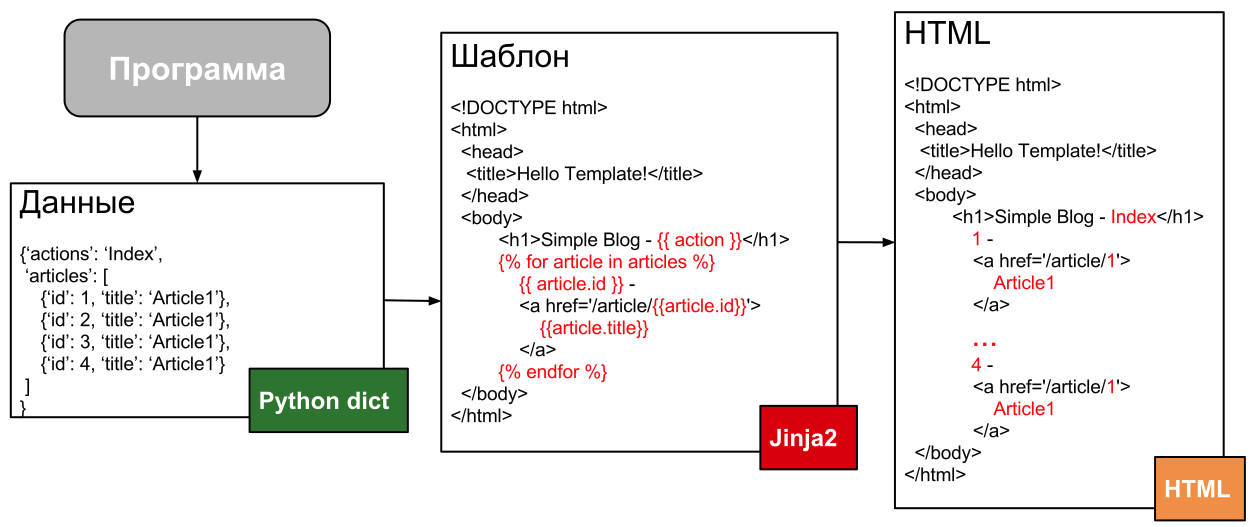
\includegraphics[width=\textwidth,height=\textheight,keepaspectratio]{media/template.png}
  \end{center}

\end{frame}


\end{document}
